\setlength{\parindent}{2ex}
\begin{chapter}{Introduction}\label{chapter:introduction}
  Visual information has been a crucial source of scientific information throughout history (in addition to being a rich source of creative and artistic expression).  
  The word ``observation'' generally connotes close visual scrutiny, and its use as a catch-all for the measured verification of a hypothesis in the scientific method exemplifies the central role of visual perception in science.
  Many famous experiments rely on careful descriptions of viewed observations; for example, Gregor Mendel visually observed the colors of various organs in his famous experiments on hybridized peas to develop the early principles of genetics.
  With the advent of the camera and photosensitive chemistry, high fidelity recording of visual observations became possible and proved immensely useful to science.
  Arthur Eddington's famous celestial observations in the early 20th century which provided the first experimental verification of Albert Einstein's general theory of relativity were recorded on photographs taken during a solar eclipse.
  The richness of raw data content in recorded images and our human propensity to digest visual information -- the proof is in the picture, so to say -- make recorded visual data in images a compelling source of scientific evidence and information.
  The ever-progressing technology in optical science and engineering are rapidly increasing the amount of data in each image; yet, it is precisely this extreme density of data that makes a \emph{quantitative} analysis of images challenging.

  Images, when viewed quantitatively, can be described as the response of the incidence of light and the subsequent exchange of energy on a grid of regularly spaced points, which we refer to as pixels.
  The raw volume of recorded data is usually very large.
  For instance, astronomical images such as those captured by interstellar robotic probes are digitized on a pixel grid typically $800 \times 800$ or higher, that measures the counts of captured photons on an array of detectors referred to as a charged coupled device (CCD) array \citep{voyager}.
  In medical imaging, computed tomography is an imaging process whereby a three dimensional image is constructed from a series of axial measurements of attenuation of electromagnetic radiation. 
  The additional dimension to the grid multiplicatively increases the data.
  Of primary focus in this work are pulsed X-ray measurements, referred to as radiographs, that are used as an experimental diagnostics of high-energy physics experiments.  
  In this case, X-rays are pulsed through a contained experiment, then the attenuated X-rays excitep a crystal that responds by luminescing visible light at an intensity related directly to the energy of the attenuated wave-front.  
  The light is then captured on a high resolution CCD array on the order of $1028 \times 1028$ pixels.

  A quantitative analysis of image data must take into account pixel to pixel dependence.
  That is, the measured values at one pixel depends heavily on adjacent or neighboring pixels, thus, one expects the measured data to be highly correlated.
  From a statistical point of view, explicitly accounting for spatial correlation in data is a very complex problem, and one of the first substantive achievements was by Julian Besag in 1974 with his seminal paper ``Spatial Interaction and the Statistical Analysis of Lattice Systems,'' \citep{besag1974}.
  The relatively recent date of this publication (in mathematical terms) coupled with the prevalence of image data prior to this, hints that the requisite tools for a rigorous statistical analysis require modern mathematical theory and state of the art computation.
  The development over the past several decades in this area has inspired a wealth of theory and computational tools, but is far from complete.
  Moreover, a broad field of scientific disciplines have considered image data, or more generally spatially correlated data, in one way or another; fields such as astronomy, astrophysics, biology, medicine, geology, computer science, and nuclear physics to name a few.
  Each have a unique perspective on the problem, and a vast literature on the subject \citep{cressie1993statistics,andOthers} has accumulated.
  Although much work has been done, it is still a very active research area and is far from the level of consensus and understanding that analysis of independently sampled data has achieved. 
  But it is precisely this lack of independence that makes an image interesting -- independent image data is ``gray noise'' from which one can only infer the average measured pixel.
  The aim of this work is to develop and adapt current models and methods for estimation and quantifying uncertainty to a small component of image analysis related specifically to the \emph{system for capturing images}.
  Understanding this component is a preliminary step to developing methods for quantitatively analyzing the images themselves.

\section{Modeling blur with the point spread function}
  
  One major component of the spatial relationship of neighboring pixels of an image is due to blur from the imaging instrumentation.
  That is, under the assumption that arbitrary images are measured by a consistently modeled system, what contribution does this system have on how pixels are related, and how can we quantify this relationship?
  A widely used model for blurring \citep{hansen2006,jain1989,vogel2002,andOthers} expresses this relationship through a point-wise integral product with a function that describes interaction with neighboring points, e.g.
  \begin{equation}\label{eq:generalPsf}
    b(x,y) = \iint_{\Omega} k(x,y,s,t) f(s,t)\,dsdt
  \end{equation}
  where $b(x,y)$ are the quantitative measurements of the blurred image, $f(s,t)$ represents the ideal un-blurred image with domain $\Omega$, and $k$ is a function that describes the blur for each given $(x,y)$.
  Informally, the function ``weights'' the other points in the image, and the integration ``averages'' the weighted values of the ideal image $f(s,t)$.
  The form of the weighting function is guided by optical principles and the physics of the system that generally dictate that, for fixed $(x,y)$, $k(x,y,\cdot,\cdot)$ is concentrated (in the measured or integrated sense) at $(x,y)$ and continuously decays as the distance from $(s,t)$ to $(x,y)$ increases.
  In this sense, the weighting effect of \eqref{eq:generalPsf} ``spreads'' outward from $(x,y)$, hence, is referred to as the point spread function (PSF).

  Under the additional assumption that the effect of blur is invariant to translations of $(x,y)$, the dimension of the domain of the PSF reduces from four to two (we still denote it by $k$) and 
blur at $(x,y)$ is given by integrating against translates of $k(x,y)$, i.e.
\begin{equation}\label{eq:convolutionDeterministic}
  b(x,y) = \iint_{\Omega} k(x-s,y-t) f(s,t)\,dsdt.
\end{equation}
  The integral product in \eqref{eq:generalPsf} is called the convolution of $f$ by $k$.
  The assumptions for modeling blur in this form are quite common, and methods that mitigate the effect of blur are often referred to deconvolution techniques.
  Note that a change of variables by $s'=x-s$ and $t'=y-t$ results in a convolution of $k$ by $f$, which is to say that convolution, as an operation, is symmetric.
  This dual relationship between the PSF and the image will allow us to use the framework and tools of deconvolution for the problem of PSF estimation.

  Typically, deconvolution methods assume the form of the PSF can be accurately described by modeling the imaging system \citep{jain1989}, but for complex imaging systems such as the one described for X-ray radiography, this is not realistic.
  Instead, if the imaging system is designed so that repeated images can be taken under consistent conditions, then by convolution symmetry, the blurring of a \emph{known calibration image} can be cast as deconvolving the PSF from the ideal $f$ corresponding to the known image.
  A direct estimate can be obtained by imaging a bright point source, which approximates the impulse response to \eqref{eq:convolutionDeterministic}.
  In astronomical imaging, the point source can be a bright distant star, or in a controlled setting where visible light is measured, a focused laser beam provides a good point source estimate.
  However, in the spectral regime of high frequency X-rays, the problem of focusing high frequency light is notoriously difficult and usually impractical in the situations of interest, so a point source estimate of the PSF is usually unavailable at these frequencies.
  Instead, the system response of a uniformly opaque calibration object with a simple geometry can be measured.
  Under the assumption that the object attenuates X-rays sufficiently so that the ideal image is given by an indicator function for a known set $E \subseteq \Omega$, then we can form a deconvolution problem that exploits our control over the geometry of $E$.
  When the calibration object is a vertical edge at a known fixed location in the imaging plane, then $E$ is the half plane, and its characteristic function depends only on $s$ and is given by $f(s) = 1$ if $s\ge0$ and $f(s)=0$ if $s <0$. 
  The model for blur in \ref{eq:convolutionDeterministic} reduces to
\begin{equation}\label{eq:psfForwardModelDeterministic},
  b(x,y) = \iint_{\Omega} k(s,t) f(x-s)dsdt. 
\end{equation}
  Note that $b$ no longer depends on $y$, hence the model output provides data only in the horizontal dimension.
  This leads to the problem of estimating $k$ from $b$ in \eqref{eq:psfForwardModelDeterministic} being underdetermined, since there are generally many distinct $k$ that can result in the same output $b$, so the problem must be further constrained. 
  A natural way to reduce the dimensionality of $k$ is to assume it has radial symmetry and can be uniquely determined a radial profile.
  That is, there exists a function $g$ defined on $\Omega_1$ a subset of $(0,\infty)$ so that $k(s,t) = g(\sqrt{s^2 + t^2})$.  

  Hence, when one believes that the PSF of their system is radially symmetric, a calibration object of the type in \cref{fig:edgeData} is sufficient to reconstruct the radial profile of the PSF and can be done in one dimension.

  Finally, the measurements of the imaging system are generally not deterministic and are subject to measurement noise.
  Precisely modeling the stochastic effect of measurement error is system dependent and can be quite complicated.
  In the X-ray radiography example, uncertainty can enter into the system at the luminescing crystal response, at the counts of CCD array, or through the electrical transmission of the signal.
  Appealing generally to central limit theorems, we model the stochastic measurement effect in aggregate as independent Gaussian noise with zero mean and unknown variance.  
  The complete description of the model from which the PSF will be estimated is
\begin{equation}\label{eq:psfForwardModelStochastic} 
  b(x) = \iint_{\Omega} k(s,t) f(x-s)dsdt + \eps_x  
\end{equation}
  where each $\eps_x \sim N(0,\sigma^2)$ and independently (in $x$) for some unknown variance $\sigma^2$.

  The discussion thus far has been somewhat informal, as we have not defined a space for the solution or the output and a rigorous treatment will be given in Chapter 2.

\section{An edge blurred with a radially symmetric point spread function}

It is common to reduce the dimensionality of the reconstruction problem by assuming a parametric form of the PSF, and many of the most common models for the PSF are radially symmetric \citep{doering1992,jain1989,kundur1996blind,watson1993}.
Here, we retain the assumption of radial symmetry, but do not assume a parametric form. Thus, solving (\ref{psfForwardModel}) can be recast on the one-dimensional radial profile, $x$, of $k$.

The radial profile is $x:(0,\infty)\to \RR$ such that $k(s',t') = x( \sqrt{{s'}^2 + {t'}^2})$, then using the change of variables $s' = r\cos v, t'= r\sin v$ in (\ref{psfForwardModel}) and integrating in $t$ results in the integral operator on the radial profile
\begin{equation}\label{eq:fredholmEquation}
  b(s) = \int_0^\infty x(r) g(s,r) r dr, 
\end{equation}
where
\begin{equation}
  g(s,r) = \left\{\begin{array}{lr}
    0 & s < - r\\
    2(\pi - \acos(x/r)) & |s| < r\\
    2\pi &  s> r
  \end{array}\right..  \label{g_form}
\end{equation}
Observe that $g(s,r)$ is continuous (although it has a discontinuity in its partial derivatives across $r=s$),
so (\ref{fredholmEquation}) is a Fredholm equation of the first kind, and therefore a linear inverse problem of the form (\ref{eq:lip}).
Moreover, since the operator is compact, the problem is ill-posed and its discretization results in a matrix with singular values that cluster near zero \citep{Han10}.

\section{Radial profile reconstruction as an ill-posed inverse problem}

  Estimating $k$ from measurements $b$ in \ref{eq:psfForwardModelDeterministic} is referred to as an inverse problem. 
  There is much in the literature of inverse problems related to image deconvolution, and due to the dual nature of the PSF reconstruction problem, we build upon the work there.
  In particular, we will take a Bayesian approach to the inverse problem from which uncertainties in the estimate can quantified.
  These methods have been the subject of much recent research (see the books \citep{Calvetti,Kaipo,Stuart}) and will be briefly outlined in the following chapter.
  
\section{Organization}
  In the next chapter, we will give a basic outline of Bayesian estimation techniques for the problem of PSF reconstruction.
  Primarily, we will develop the theoretical framework of how inference can be carried out on the radial profile of the PSF, rather than the PSF itself.
  Chapter 2 will be mainly theoretical.
  Chapter 3 will give details on how to carry out the estimation on a computer.
  There we will deal with how to discretely represent each of the necessary components in the estimation problem.
  In Chapter 4, we will then motivate and present the design of a detailed algorithm for carrying out the estimation outlined in Chapter 2.
  Finally, in Chapter 5, we present the results of an implementation on synthetically derived data and on measured data from a high-energy X-ray imaging system at the U.S.~Department of Energy's Nevada National Security Site.
  We will end with a discussion of conclusions and possible future work.


\begin{figure}
  \begin{center}
    \begin{tikzpicture}[scale=.8,every node/.style={minimum size=1cm},on grid]
      \def\myxslant{0.1}
      \def\myyslant{-0.4}

	\begin{scope}[
		xshift=40,
		every node/.append style={
		xslant=\myxslant,yslant=\myyslant},xslant=\myxslant,yslant=\myyslant
	]
	\draw (0,0) rectangle (2.8,2.2);
%	\draw[fill=black] (1,0) rectangle (2.8,2.2);
	\end{scope}

	\begin{scope}[
		yshift=-20,
		every node/.append style={xslant=\myxslant,yslant=\myyslant},
		xslant=\myxslant,yslant=\myyslant
	]
	\draw[x=.314cm,y=.2cm,z=.2cm,thick,-latex,red] (0,0,0)
	  sin ++(0,1,1) cos ++(0,-1,1) sin ++(0,-1,1) cos ++(0,1,1)
	  sin ++(0,1,1) cos ++(0,-1,1) sin ++(0,-1,1) cos ++(0,1,1)
	  sin ++(0,1,1) cos ++(0,-1,1) sin ++(0,-1,1) cos ++(0,1,1);
	\draw[x=.314cm,y=.2cm,z=.2cm,thick,-latex,red] (-2,0,0)
	  sin ++(0,1,1) cos ++(0,-1,1) sin ++(0,-1,1) cos ++(0,1,1)
	  sin ++(0,1,1) cos ++(0,-1,1) sin ++(0,-1,1) cos ++(0,1,1)
	  sin ++(0,1,1) cos ++(0,-1,1) sin ++(0,-1,1) cos ++(0,1,1);
	\draw[x=.314cm,y=.2cm,z=.2cm,thick,-latex,red] (-4,0,0)
	  sin ++(0,1,1) cos ++(0,-1,1) sin ++(0,-1,1) cos ++(0,1,1)
	  sin ++(0,1,1) cos ++(0,-1,1) sin ++(0,-1,1) cos ++(0,1,1)
	  sin ++(0,1,1) cos ++(0,-1,1) sin ++(0,-1,1) cos ++(0,1,1);

	\pgfmathsetmacro{\cubex}{2}
	\pgfmathsetmacro{\cubey}{2.5}
	\pgfmathsetmacro{\cubez}{1}
	\draw[black,fill=gray,opacity=.75] (3.7,3,0) -- ++(-\cubex,0,0) -- ++(0,-\cubey,0) -- ++(\cubex,0,0) -- cycle;
	\draw[black,fill=gray,opacity=.75] (3.7,3,0) -- ++(0,0,-\cubez) -- ++(0,-\cubey,0) -- ++(0,0,\cubez) -- cycle;
	\draw[black,fill=gray,opacity=.75] (3.7,3,0) -- ++(-\cubex,0,0) -- ++(0,0,-\cubez) -- ++(\cubex,0,0) -- cycle;

	\draw[x=.314cm,y=.2cm,z=.2cm,thick,-latex,red] (4,0,0)
	  sin ++(0,1,1) cos ++(0,-1,1) sin ++(0,-1,1) cos ++(0,1,1)
	  sin ++(0,1,1) cos ++(0,-1,1) sin ++(0,-1,1) cos ++(0,1,1);
	\draw[x=.314cm,y=.2cm,z=.2cm,thick,-latex,red] (2,0,0)
	  sin ++(0,1,1) cos ++(0,-1,1) sin ++(0,-1,1) cos ++(0,1,1)
	  sin ++(0,1,1) cos ++(0,-1,1) sin ++(0,-1,1) cos ++(0,1,1);
	\end{scope}

	\begin{scope}[
		xshift=180,
		every node/.append style={xslant=\myxslant,yslant=\myyslant},
		xslant=\myxslant,yslant=\myyslant
	]
	    \draw (0,0) rectangle (2.8,2.2);
	    \tikzfading[name=fade left,left color = transparent!100,right color = transparent!0]
	    \draw[path fading=fade left,fading transform={rotate=-30},fill=black] (.9,0) rectangle (1,2.2);
	    \draw[fill=black] (1,0) rectangle (2.8,2.2);
	\end{scope}

	\begin{scope}[
		xshift=300,
		every node/.append style={xslant=\myxslant,yslant=\myyslant},
		xslant=\myxslant,yslant=\myyslant
		]
	    \draw (0,0) rectangle (2.8,2.2);
	    \tikzfading[name=fade left,left color = transparent!100,right color = transparent!0]
	    \draw[path fading=fade left,fading transform={rotate=-30},fill=black] (.9,0) rectangle (1,2.2);
	    \draw[fill=black] (1,0) rectangle (2.8,2.2);
	    \draw[step=1mm, black] (0,0) grid (2.8,2.2); %defining grids
	\end{scope}
	

    %    %putting arrows and labels:
	\node at (2,2.5) (label1) {Opaque Edge};
	\draw[-latex,thick] (2,-2) to node[below] {Image System Response} (7.5,-2);
	\node at (4.65,-3.4) (math1) {$\displaystyle{b(x)=\iint_{\Omega} k(s,t) f(x-s)\,dsdt}$};

	\node at (7,2.5) (label3) {Blurred Profile};

	\node at (12,2.5) (label2) {Recorded Data};
	\draw[-latex,thick] (9,-2) to node[below]{Measurement error} (13.2,-2);
	\node at (11,-3.4) (math1) {$+\eps_x \sim N(0, \sigma^2)$};

    \end{tikzpicture}
  \caption{ A schematic of the measurement model for an X-Ray image of an edge. An opaque block aligned with the imaging plane blocks light on the half plane to produce a blurred edge.}\label{fig:edgePicture}
\end{center}
\end{figure}

\begin{figure}
\begin{center}
  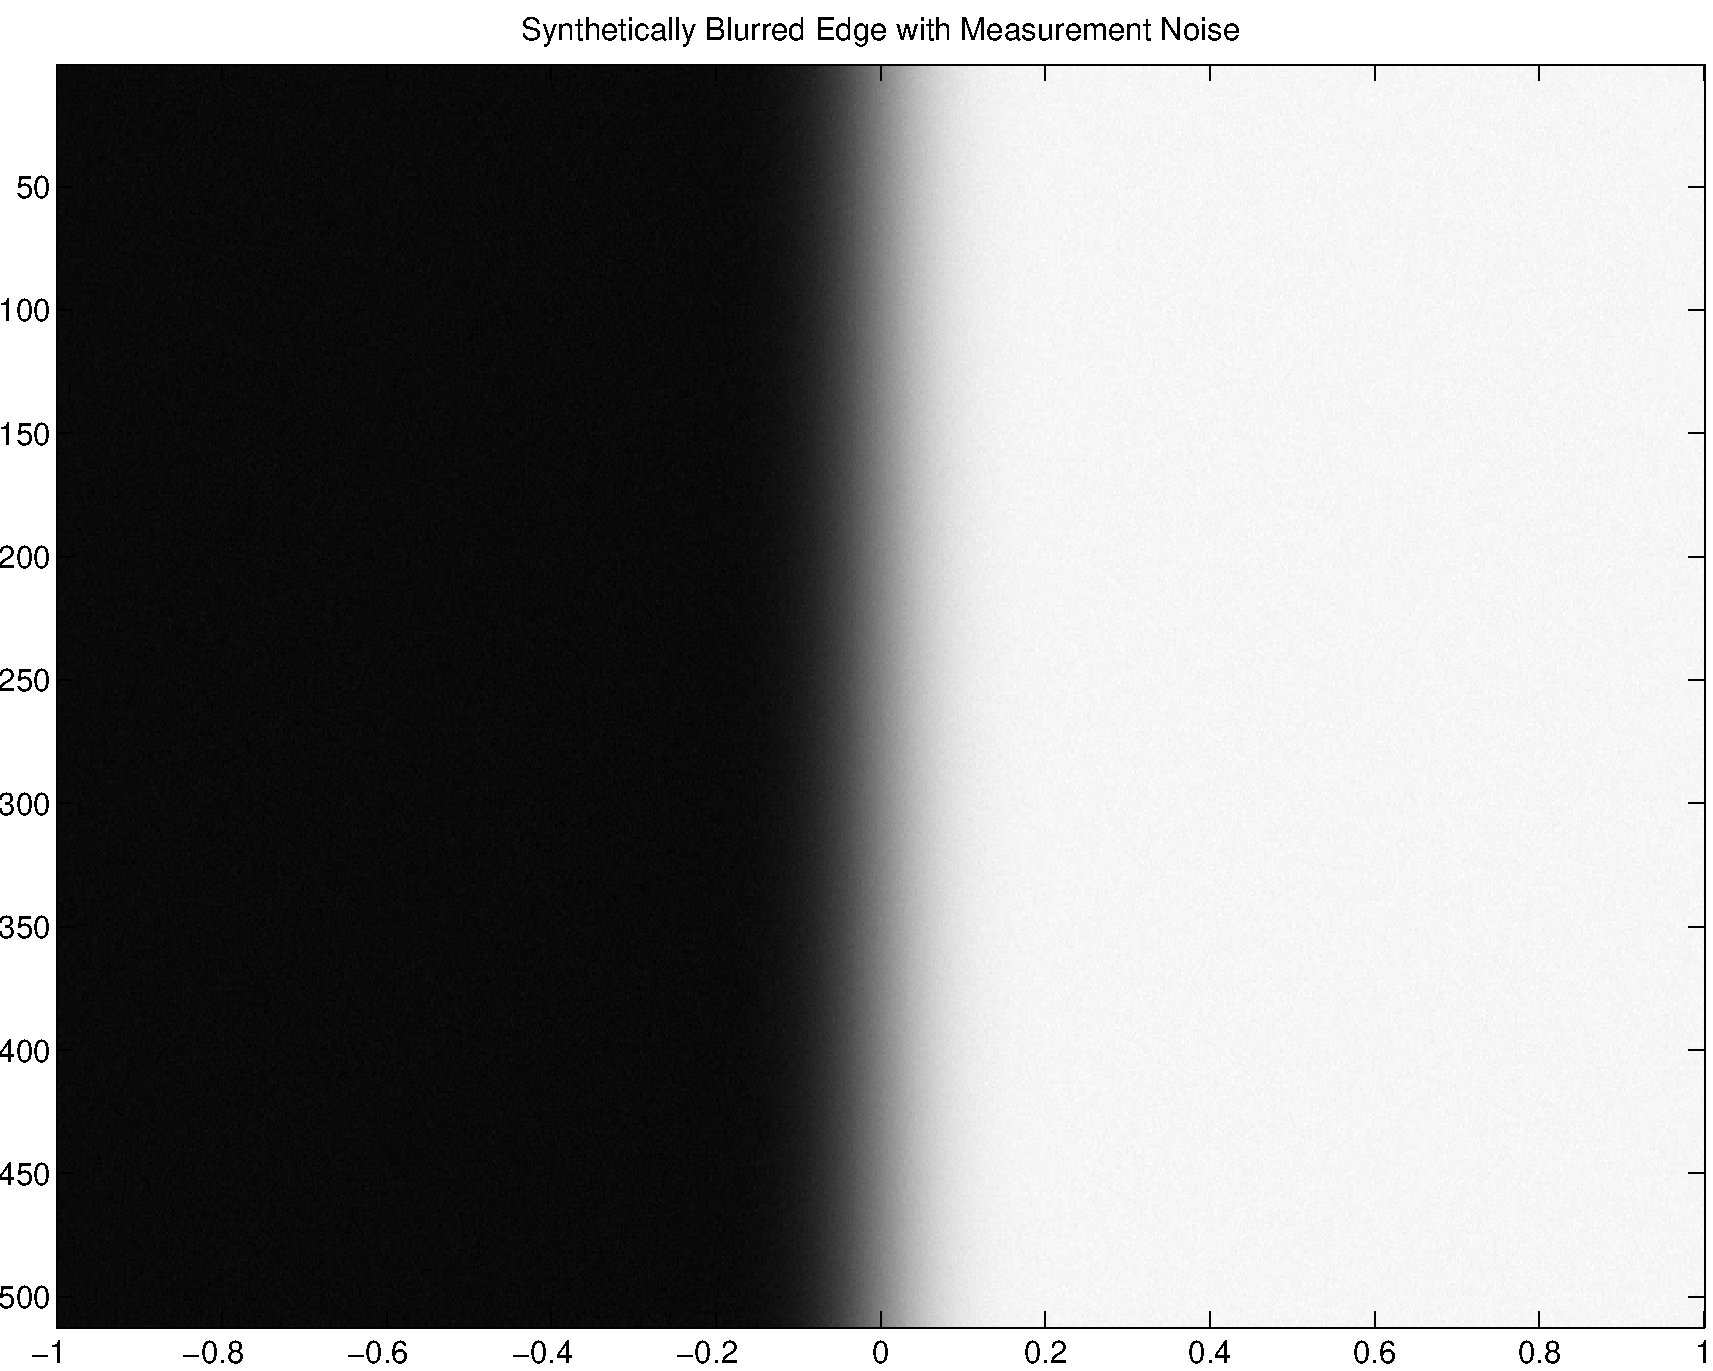
\includegraphics[width=.45\textwidth]{figures/blurredEdgeData.pdf}
  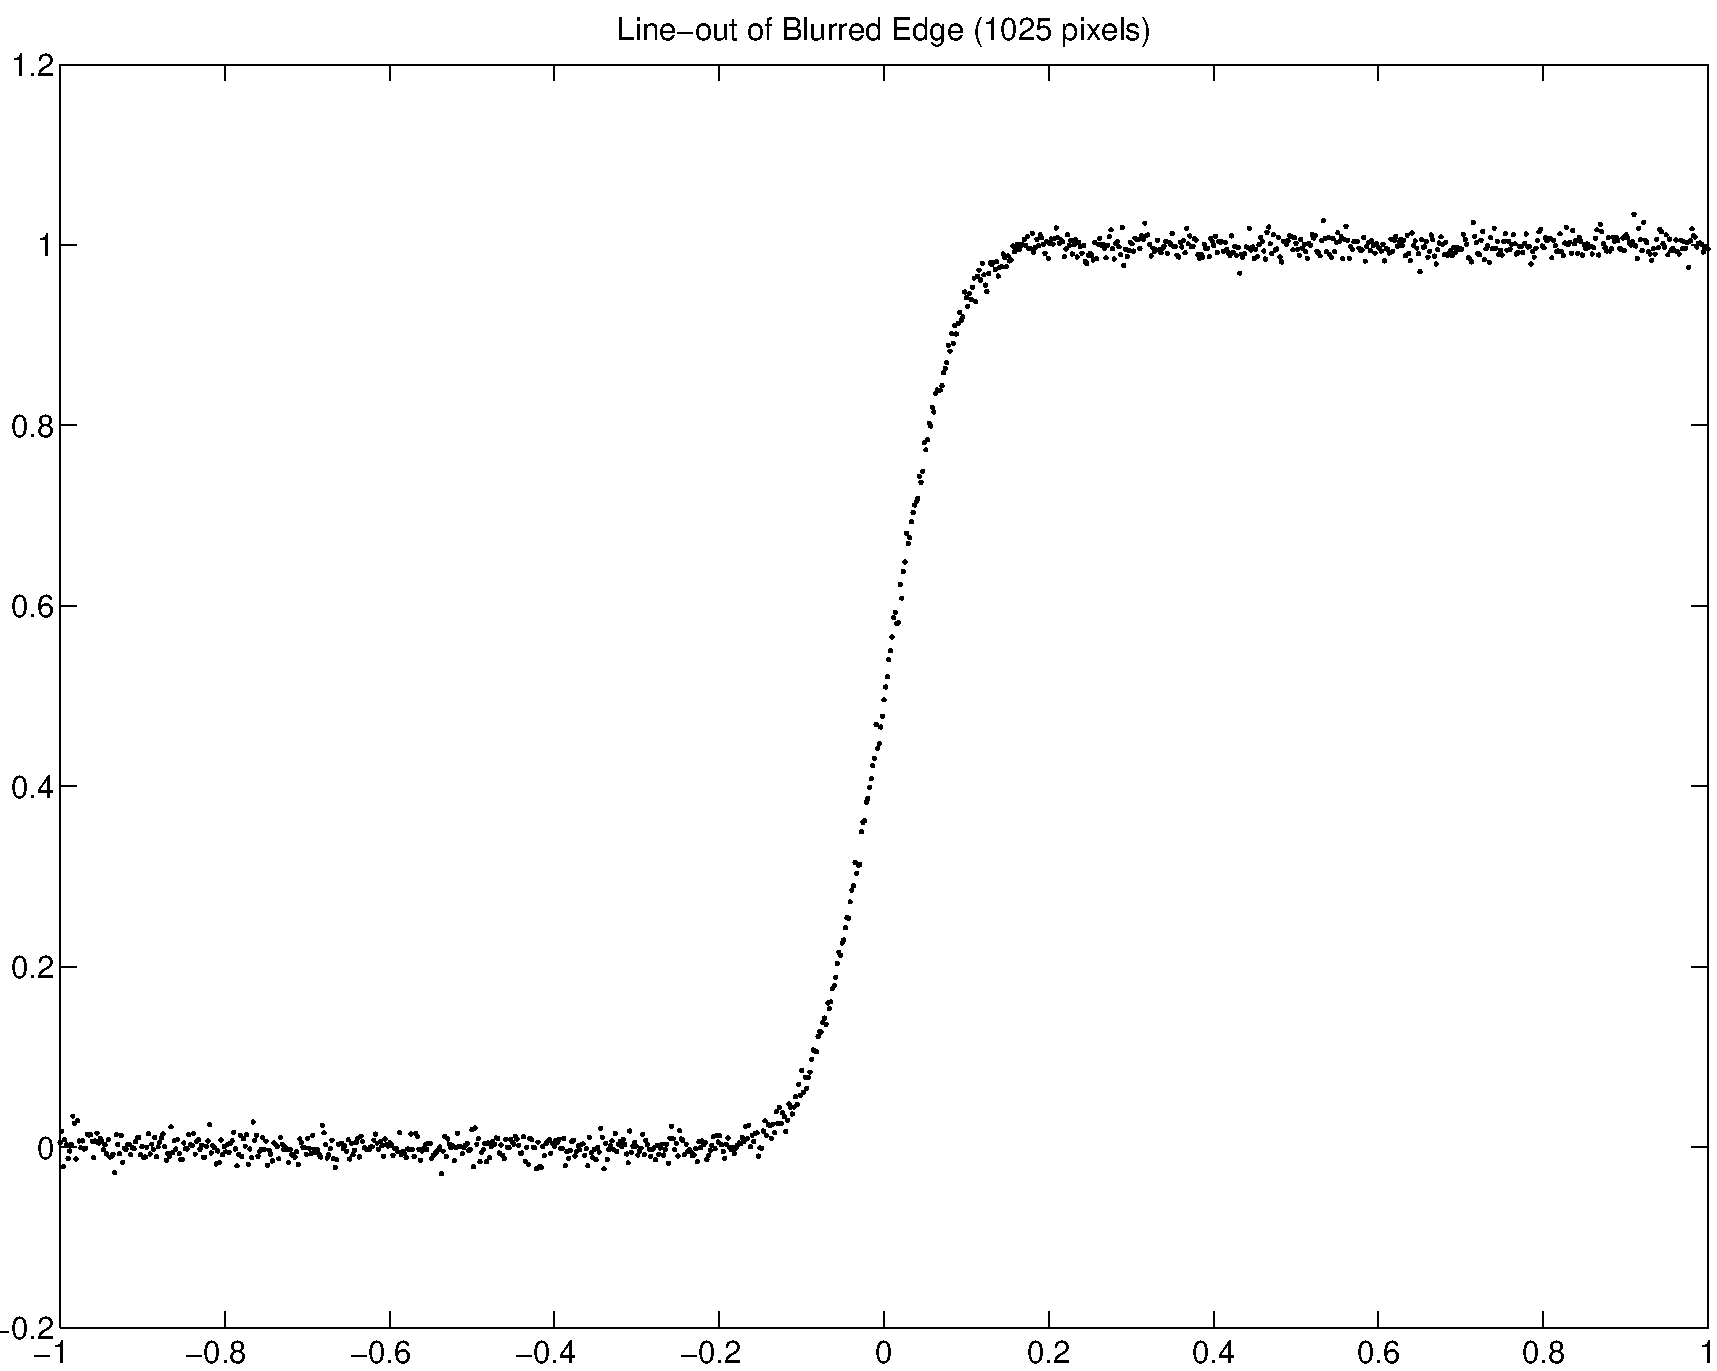
\includegraphics[width=.45\textwidth]{figures/psfLineoutData.pdf}
  \caption{A synthetically blurred edge with simulated measurement error and a line-out (horizontal cross-section) from the data.} \label{fig:edgeData}
\end{center}
\end{figure}

\end{chapter}
